\begin{document}

\chapter{Classification Pipeline Time and Space Requirements Analysis}

This appendix aims to give an intuition of how the classification pipeline would actually behave in a real world scenario. I firstly define the classification time of N nodes, using pre-trained models, by the following formulas: \\

    \begin{equation}
        \centering
        \text{TT = MLT  + N * CT}
    \end{equation}
    
    where: \\
    TT - total time for classifying N nodes. \\
    MLT - total times for all the pre-trained models involved to be loaded into memory. \\
    CT - total classification time of a file. \\
    
    \begin{equation}
        \centering
        \text{MLT = CNN LT + MLP LT + LRG LT} 
    \end{equation}
    
    where: \\
    CNN LT - loading time of the trained convolutioanl neural network \\
    MLP MT - loading time of the trained mutilayer perceptron \\
    LRG LT - loading time of the trained logistic regression model \\
    
    \begin{equation}
        \text{CT = Content CT + Context CT + Stacked Ensemble CT}
    \end{equation} \label{CT}
    
    where: \\
    Content CT - time for the content pipeline to classify a file \\
    Context CT - time for the context pipeline to classify a file \\
    Stacked Ensemble CT - time for the logistic regression (LRG) to classify predictions of the base classifiers \\
    
    The way in which Equation \ref{CT}.3 splits even further, as well as how average timings are computed for each subtask, are clearly illustrated in Figure \ref{timings}. In this figure the following abbreviations stand for: PT - prediction time, FPT -feature processing time, BFS - time for performing a breadth first search query on the neo4j database (for a graph with ID = 3 and HD = 4), FET - features extraction time for a single database node and AGS - average graph size. \\
    
\begin{figure}[H]
  \centering
  \centerline{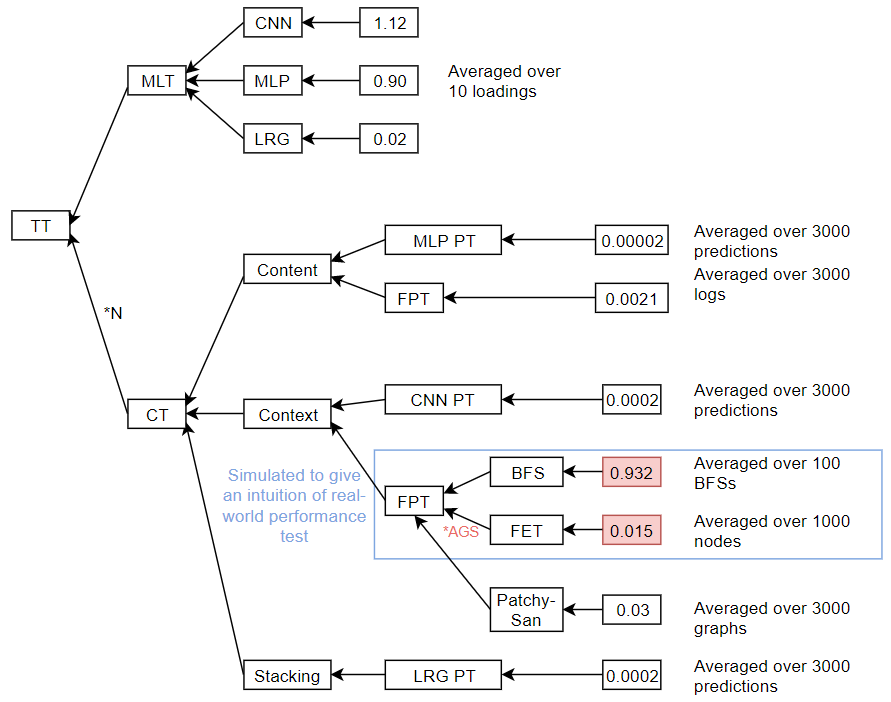
\includegraphics[scale=0.6]{Images/timings.png}}
  \caption{Diagram illustrating all components considered for calculating total service time. Highlighted in red is the neo4j querying bottleneck. All times are specified in seconds.}
  \label{timings}
\end{figure}

Finally, we take into account that AGS is roughly equal to 30 nodes, in the synthetic dataset used for evaluation. Thus, one can compute the average time for classifying 1000 files to be approximately 1414.52s, out of which 1328s are spent querying the neo4j database. This highlights a massive bottleneck that limits pipeline's performance. Deployment of such a pipeline would require further thought and work in order to test different approaches to solve this issue. \\

With respect to space requirements, the input graphs and files' contents must not be all held in memory at the same time, as they can be presented one by one to the already trained models. The space complexity is hence dominated by the dimensions of the NNs implemented. \\

\end{document}